\begin{document}% document begins
%
%
\subsubsection{Problem and Analysis}
%
\begin{adjmulticols}{2}{\innerMar}{\outerMar}
%\begin{adjmulticols}{2}{-.5in}{-.5in}
  %
\paragraph{Background}
%
\noindent Allegan County GIS Services builds and maintains the geographic dataset used in workflows in and out of county government.
%
\paragraph{Statement of Problem}
%
\noindent Geographic data must be be both maintained and shared.  Data is maintained by Equalization and GIS Services.  Data is shared with EH, EQ, Dispatch and the public.
%
\paragraph{Analysis}
%
\noindent Here is where analysis of this problem goes
%
%\end{multicols}
\end{adjmulticols}
%
\clearpage
    %
\subsubsection{Design}

\paragraph[Overview]{Overview}


% Single Figure
%
\marginpar{\color{graphicOrange}\textbf{Forfeiture Parcels} is used through the workflow}
\vspace{-.2in}

\begin{figure}[h!]
\centering
    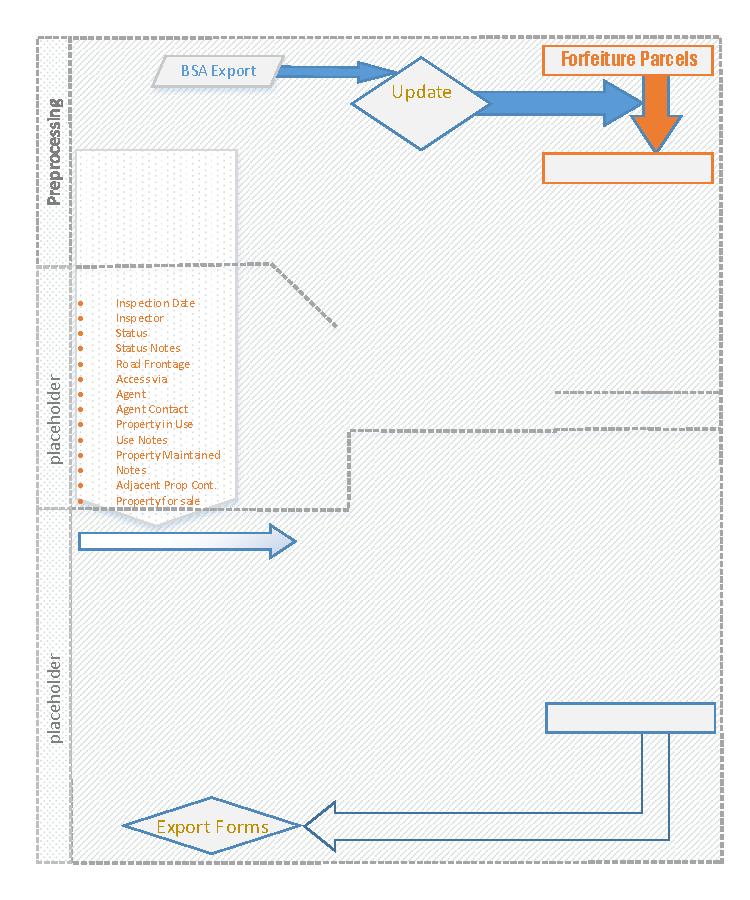
\includegraphics[width=1\textwidth]{ProjectDesign}
\vspace{-.2in}

\caption{Project Design}
\end{figure}
%\marginpar[]{$\Rightarrow$}
\clearpage








\subsection[Production Data]{Production Data AC PRO}
\medskip







\subsubsection{Domains}
%
\paragraph[Directory Location]{Directory Location\texorpdfstring{\\}{}}
%
\noindent Manged at this location:
%
\begin{figure}[h!]
\centering
    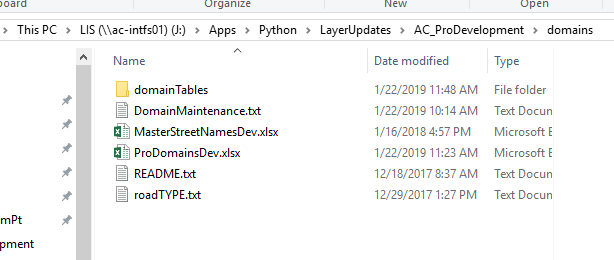
\includegraphics[width=.6\textwidth]{layerUpdatesFileLocation.PNG}

\caption{Directory Location of Workspace}
\end{figure}
%
%
%

\subparagraph[Domain Documentation]{Domain Documentation\texorpdfstring{\\}{}}
\noindent This is where...
%\vspace{.1in}

{\Large $\Rightarrow$ Push the Configure Button}


\end{document}
